%
% PROJECT: <ETD> Electronic Thesis and Dissertation Initiative
%   TITLE: LaTeX report template for ETDs in LaTeX
%  AUTHOR: Neill Kipp, nkipp@vt.edu
%     URL: http://etd.vt.edu/latex/
% SAVE AS: etd.tex
% REVISED: September 6, 1997 [GMc 8/30/10]
% 

% Instructions: Remove the data from this document and replace it with your own,
% keeping the style and formatting information intact.  More instructions
% appear on the Web site listed above.

\documentclass[12pt]{report}

\setlength{\textwidth}{6.5in}
\setlength{\textheight}{8.5in}
\setlength{\evensidemargin}{0in}
\setlength{\oddsidemargin}{0in}
\setlength{\topmargin}{0in}

\setlength{\parindent}{0pt}
\setlength{\parskip}{0.1in}

% Uncomment for double-spaced document.
% \renewcommand{\baselinestretch}{2}
\usepackage{graphicx}
\usepackage{epstopdf}
\usepackage{listings}
\usepackage{color}
\usepackage{tikz}
% \usepackage{epsf}

\begin{document}

\thispagestyle{empty}
\pagenumbering{roman}
\begin{center}

% TITLE
{\Large 
Replication of Concurrent Applications in a Shared Memory Multikernel
}

\vfill

Yuzhong Wen

\vfill

Thesis submitted to the Faculty of the \\
Virginia Polytechnic Institute and State University \\
in partial fulfillment of the requirements for the degree of

\vfill

Master of Science \\
in \\
Computer Science and Application

\vfill

Binoy Ravindran, Chair \\
Ali R. Butt Co-Chair \\
Dongyoon Lee

\vfill

June 17, 2016 \\
Blacksburg, Virginia

\vfill

Keywords: blah, blah
\\
Copyright 2016, Yuzhong Wen

\end{center}

\pagebreak

\thispagestyle{empty}
\begin{center}

{\large Replication of Concurrent Applications in a Shared Memory Multikernel}

\vfill

Yuzhong Wen

\vfill

(ABSTRACT)

\vfill

\end{center}

Lorem ipsum dolor sit amet, consectetur adipiscing elit. Nunc nec elit molestie, mattis mi a, consequat arcu. Fusce venenatis rhoncus elit. Morbi ornare, libero a bibendum pretium, nibh orci tristique mauris, in suscipit mauris nibh ac metus. Nullam in sem vitae nisi aliquet iaculis in a nibh. Aliquam lobortis quis turpis ut tempus. Sed eu sapien eu nisi placerat viverra pharetra eu turpis. Mauris placerat massa mi, auctor facilisis sem consequat in. Pellentesque sollicitudin placerat mi quis rhoncus. In euismod lorem semper, scelerisque leo et, dapibus diam. Suspendisse augue dui, placerat at finibus a, cursus vitae erat. Nam accumsan magna vitae lorem tincidunt, et rhoncus elit consequat.

Suspendisse ut tellus at ex suscipit sollicitudin ut ut elit. Nam malesuada molestie elit eget luctus. Donec id quam ullamcorper, aliquam mauris at, congue felis. Nunc dapibus dui sit amet nisl laoreet, eget rhoncus est tempor. Mauris in blandit mauris. Aenean vitae ipsum lacinia, blandit turpis et, feugiat purus. Mauris in finibus quam, ac dictum lorem. Nam dignissim luctus ante. Suspendisse risus felis, imperdiet a lobortis sed, suscipit ac dui. Nullam fermentum velit eu congue dictum. Pellentesque tempor dui vel nisl tristique, non sollicitudin odio elementum. In ultricies elementum mattis.

Vestibulum eget imperdiet eros. Proin bibendum sit amet felis quis dignissim. Aliquam convallis mauris ut sapien gravida, eu consequat lacus dignissim. Vivamus porttitor hendrerit nisl, sit amet suscipit lorem vestibulum ut. Donec id tellus condimentum, sollicitudin sapien vel, lobortis nulla. Donec et elit quis est tempor semper. Aliquam erat volutpat. In nec consectetur dui. Nullam aliquam diam at eros ultrices vehicula. Nulla nibh ex, condimentum vitae nisl sed, aliquet ultricies sapien. Suspendisse potenti. Suspendisse pellentesque tincidunt facilisis. Morbi sodales vulputate ex malesuada molestie. Vestibulum eget placerat nunc.
\vfill

% GRANT INFORMATION

This work is supported by AFOSR under the grant FA9550-14-1-0163.  Any opinions, findings, and conclusions expressed in this thesis are those of the author and do not necessarily reflect the views of AFOSR.

\pagebreak

% Dedication and Acknowledgments are both optional
% \chapter*{Dedication}
% \chapter*{Acknowledgments}

\tableofcontents
\pagebreak

\listoffigures
\pagebreak

\listoftables
\pagebreak

\pagenumbering{arabic}
\pagestyle{myheadings}

\newcommand{\detstart}{\_\_det\_start}
\newcommand{\detend}{\_\_det\_end}
\newcommand{\dettick}{\_\_det\_tick}

\chapter{Introduction}
% 1. single machine replication
% 2. state machine replication
% 2.1 weak determinism, total order of synchronization primitives.
% 3. contribution
% 3.1 deterministic execution and schedule replication inside kernel
% 3.2 fully transparent, minimal modification to application
% 3.3 comparision that sched rep is better

% cite a bunch of intra-machine solutions
% Hypervisor-based Fault-tolerance
% Operating System Support for Redundant Multithreading
% Tardigrade: Leveraging Lightweight Virtual Machines to Easily and Efficiently Construct Fault-Tolerant Services


%With increasing number of CPU cores and memory size, multi-threaded and multi-process applications are widely adopt to extract the full potential of such high performance multi-core machines. 

Nowadays semiconductor industry pushes the CPU core count day by day. Having a computer system with high CPU core count and large memory capacity is cheaper than ever before. However with the technology advances, we still cannot ignore the fact that computer systems suffer from manifold failures time to time. Especially transient fault in a sophisticated computer system can cause memory and CPU cores to fail. Current SMP operating systems are usually fragile to such failures. A faulty device, a CPU failure or a memory damage usually lead to the entire system to crash. To be able to recovery from such severe failures, having backup machines is always a good idea. When the primary machine fails, the backup machines are set to be able to take over the previous work and carry on the services.

State machine replication (SMR) has been widely used for fault-tolerance replication . In SMR, it models the services to be replicated with a set of inputs, a set of outputs and a set of states. The replication system ensures that for a given input set, from the same initial state, the replicas can produces the same state transition which in turn leads to the same output. Such a system is able to be resilient to failures in one or more replicas (depends on how many replicas are there in the system). To provide such property, determinism is required for the state machine, otherwise state machines will get diverged in different states even with the same input set.

With the idea of SMR, there are a good amount of works that allows users to have multiple machines to act as replicas ~\cite{cui2015p}~\cite{zagorodnov2009practical}~\cite{singh2009zeno}~\cite{mao2008mencius}. While these solutions requires additional machines to do the replication, some works have explored the possibility of doing replication inside the same machine. In ~\cite{zhang2012runtime} and ~\cite{lee2010respec}, they proposed replication systems that can have a redundant execution instance along with the original one. But doing the replication inside the same OS cannot mitigate a transient fault that could fail the entire OS. To have a full stack replication that can minimize the impact of an OS failure, several works have investigated the approaches of doing replication via virtualization~\cite{bressoud1996hypervisor}~\cite{lorch2015tardigrade}~\cite{dunlap2002revirt}. However, such solutions can still suffer from the faults happen in the hypervisor.

Multi-kernel

% ~\cite{zhang2012runtime}
% A section for server applications
% Practical and Low-Overhead Masking of Failures of TCP-Based Servers

\section{Contributions}

This thesis presents the following contributions:

\begin{itemize}
\item To synchronize thread inter-leavings of replicated concurrent applications, based on Popcorn Linux, we implemented two different replication modes in the kernel, Deterministic Execution and Schedule Replication. Both of them achieved the same goal in two different directions: Deterministic Execution uses a deterministic algorithm to decide the order of execution on both primary and secondary; while Schedule Replication enforces the secondary replica to follow the non-deterministic execution order that happened previously on the primary kernel.

\item We provide a common programming interface for both replication modes. By wrapping a code section with our \detstart\ and \detend\ system calls, the execution order of wrapped sections can be the synchronized on both primary and secondary kernel. Based on this common interface, we also implemented a set of runtime supports that allows the user to run applications on our system with minimal code modification.

\item To explore the pros and cons for both replication modes, we evaluated different types of concurrent applications on our system. For computational application we had maximum 63.39\% slowdown for Deterministic Execution and maximum 36.3\% slowdown for Schedule Replication. For two web servers we had maximum 25.22\% slowdown for Deterministic Execution and maximum 1.96\% slowdown for Schedule Replication. Both replication modes achieved decent overhead for production use, but Schedule Replication is the better replication mode for most of our use case, in terms of both simplicity and lower overall overhead.
\end{itemize}

\section{Thesis Organization}
This thesis is organized as follows:

Chapter 2 presents the background of Popcorn Linux, which is the multi-kernel system we are using for building our intra-machine replication.

Chapter 3 presents our first replication mode, Deterministic Execution. 

Chapter 4 presents our second replication mode, Schedule Replication.

Chapter 5 presents the additional runtime support that we implemented to eliminate some residual non-deterministic issues, and a runtime library to simplify the application deployment on our system.

Chapter 6 shows the performance evaluation of our system on multiple concurrent real world applications.

Chapter 7 concludes the work and discusses some future works.
\chapter{Popcorn Linux Background}
Our replication prototype is built on top of Popcorn Linux ~\cite{barbalace2014popcorn}. It is a multi-kernel OS which allows a multi-core system to boot multiple Linux kernels.
% talk about multi-kernel boot here
% Put a plot of popcorn architecture here
\section{Hardware Partitioning}
In Popcorn Linux, hardware resources are partitioned into arbitrary divisions, each booted kernel instance can have the full control of its own partition.

\begin{itemize}
\item{CPU Partitioning:} Popcorn Linux is able to map an arbitrary number of CPU cores to each kernel instance. In order to get the maximum performance for concurrent applications we prefer to evenly assign CPU cores to each kernel.

\item{Memory Partitioning:} By setting the starting address and memory range during the boot time of a kernel, Popcorn Linux can also partition the memory resources for each booted kernel.
\end{itemize}

The hardware partitioning provides a very strong isolation for all the kernels and the applications running on them, which is ideal for our intra-machine fault tolerance model. Especially when the partition is done based on NUMA zones, a critical hardware error happens on one kernel's hardware partition won't get propagated to another.

\section{Inter-Kernel Messaging Layer}
Popcorn Linux comes with a high efficient messaging layer for inter-kernel communication ~\cite{shelton2013popcorn}.
% Important fact: messaging layer is strictly FIFO

\section{Popcorn Namespace}
Popcorn Linux comes with a new Linux namespace in order to isolate normal applications and replicated applications. With this namespace, the user can choose to only replicate a certain subset of applications while the rest in the system will be kept as normal. A user can enter the namespace by executing the namespace launching script, and once the user enters the Popcorn namespace, all the applications that run inside it will be replicated to the secondary kernel.
\subsection{Replicated Execution}


\subsection{FT PID}
\section{Network Stack Replication}
% Important fact: accept sequence is same on primary and replica

\chapter{Deterministic Execution}
Deterministic execution provides a property that given the same input, a multithreaded program can always generate the same output. Such a system fits perfectly for our replication purpose. As long as the primary and secondary receive the same input, the replicated application will sure end up with the same state and generate the same output.

For multi-threaded programs, an observation is that as long as the threads don't communicate with each other, the execution is sure to be deterministic\cite{devietti2009dmp}. For example, in pthread based programs, all the inter-thread communications are synchronized by pthread primitives. By making the interleaving of sychronization primitives to be deterministic, the entire program is sure to be deterministic. With this observation, some runtime deterministic solutions actually enforce determinism by trapping pthread primitives\cite{cui2013parrot}\cite{liu2011dthreads}\cite{olszewski2009kendo}. This type of deterministic system is called "Weak Deterministic System". It assumes that the applications are data race free, and only guarantee the deterministic interleaving of thread synchronization primitives such as mutex locks and condition variables. Our implementation falls into this category, but unlike other runtime deterministic systems, our runtime does not directly trap pthread primitives, but provides two system calls for programmer to define a deterministic section. The runtime maintains a global execution order, according to this order, an execution token is passed among all the tasks deterministically. Only the task with the execution token can enter the deterministic area, and the token will be held on this task only if it leaves its deterministic area.

This chapter is structured as follows:
\begin{itemize}
\item Section \ref{sec:detsched} shows the basic algorithm and programming interface of the deterministic system.
\item Section \ref{sec:logimbalance} explains the logical time imbalance problem of this algorithm and two solutions for two different cases.
\item Section \ref{sec:edeadlock} shows the case which might cause deadlock, and the solution to it.
\end{itemize}

\section{Logical Time Based Deterministic Scheduling} \label{sec:detsched}
Inspired by Kendo and Conversion, this scheduling policy maintains a logical time for each task inside the current Popcorn namespace. Our system provides three system calls for the applications to control the thread-interleaving:
\begin{itemize}
   \item \_\_det\_start: When it is called, only the task holds the minimal logical time can proceed, if several tasks have the same logical time, the one who has the smallest PID number gets the turn. If the current thread is able to proceed, this thread will be marked as "in a deterministic section".
   \item \_\_det\_end: When it is called, the system will increase the current thread's logical time by 1, and marks it as "out of a deterministic section".
   \item \_\_det\_tick: This system call comes with a parameter of an integer. When it is called, the logical time will be increased by value defined by the parameter.
\end{itemize}.

\begin{figure}
\centering
\begin{lstlisting}[numbers=left, frame=single, basicstyle=\small, breaklines]{blah}
void producer() {
    while (running){
        item = generate_item();
	    syscall(__NR_det_start);
	    pthread_mutex_lock(mutex);
	    syscall(__NR_det_end);    
	    putItem(queue, item);    
	    pthread_mutex_unlock(mutex);
    }
}

void consumer() {
    while (running){
        syscall(__NR_det_start);
        pthread_mutex_lock(mutex);
        syscall(__NR_det_end);
        item = getItem(queue);    
        pthread_mutex_unlock(mutex);		
        consume_item(item);
    }
}
\end{lstlisting}
\caption{An example use of the deterministic syscalls}
\label{fig:example}
\end{figure}
Figure~\ref{fig:example} shows an example use of the system calls. Simply wrap pthread\_mutex\_lock with \_\_det\_start and \_\_det\_end will make the acquisition of the mutex to be deterministic.

If the logical time is updated but the one has the minimal logical time is sleeping in \_\_det\_start, the one whose updates the tick will wake the sleeping one up. As long as the replicated application updates logical time in a same way on both primary and secondary, they will sure end up with the same thread interleaving. Figure~\ref{f:algorithm} shows a simplified version of this algorithm (some mutual exclusion points are omitted here).

To make an application to run in a deterministic way, one should put \_\_det\_start and \_\_det\_end around the synchronization primitives such as pthread\_mutex\_lock and pthread\_spin\_lock, so that the order of getting into critical sections is controlled under our deterministic scheduling.

\begin{figure}
\begin{lstlisting}[numbers=left, frame=single, basicstyle=\small, breaklines]{blah}
void __det_start()
{
    if (token->token != current)
        sleep(current);
    current->ft_det_state = FT_DET_ACTIVE;        
}
void __det_end()
{
    current->ft_det_state = FT_DET_INACTIVE;
    __update_tick(1);
}
void __det_tick(int tick)
{
    __update_tick(tick);
}
void __update_tick(int tick)
{
    current->tick += tick;
    token = find_task_with_min_tick(ns);
    if (is_waiting_for_toUponken(token->task))
    	wake_up(token->task);
}
\end{lstlisting}
\caption{Simplified implementation of deterministic system calls}
\label{f:algorithm}
\end{figure}

\section{Balance the Logical Time} \label{sec:logimbalance}
Only increasing the logical time by 1 at \detend\ isn't enough. With an example we show how this could break the scalability and how to mitigate this problem. In Figure~\ref{fig:imbalance}, we show a particular execution point of the producer-consumer model in the program snippet we presented in Figure~\ref{fig:example}, solid lines represents the path that is already executed. In this case, consumer reaches consumeItem with logical time 3 and has the token. Assume the real execution time of consumeItem is 10s, which means that when the consumer reaches \_\_det\_end, it would be at least 10s later, that is, the producer has to wait at \_\_det\_start for at least 10s. However we've already enforces the access order of the mutex, the execution out of the critical section should go in parallel since threads don't communicate at that point, in worst case, this kind of waiting will turn a parallel program into a serial program.

\begin{figure}
\centering
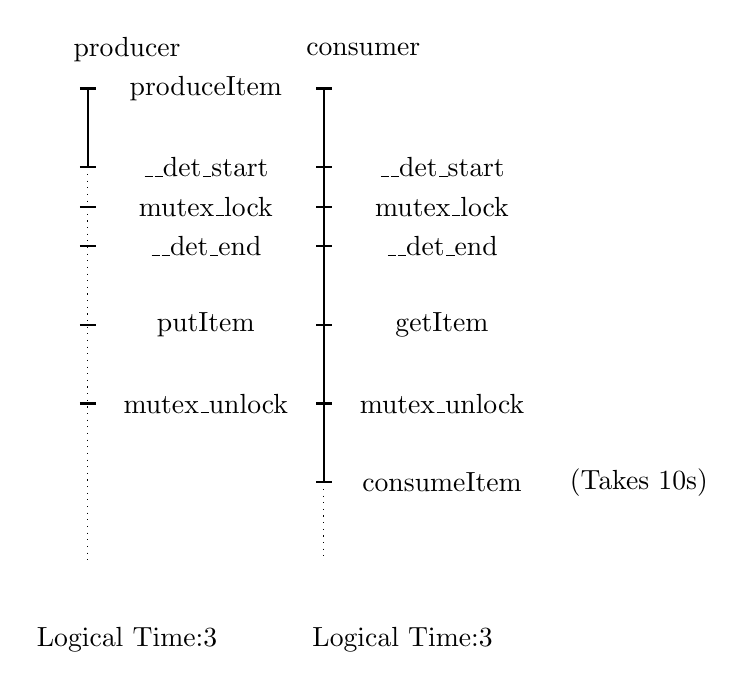
\begin{tikzpicture}
   \draw[thick] (0,4) --  (0,5); 
   \draw[dotted] (0,4) --  (0,-1);
   
   \node[align=right] at (0.5,5.5) {producer};
   \node[align=right] at (1.5,5) {produceItem};
   \draw[thick] (-0.1,5) -- (0.1,5);
   \node[align=right] at (1.5,4) {\_\_det\_start};
   \draw[thick] (-0.1,4) -- (0.1,4);
   \node[align=right] at (1.5,3.5) {mutex\_lock};
   \draw[thick] (-0.1,3.5) -- (0.1,3.5);
   \node[align=right] at (1.5,3) {\_\_det\_end};
   \draw[thick] (-0.1,3) -- (0.1,3);
   \node[align=right] at (1.5,2) {putItem};
   \draw[thick] (-0.1,2) -- (0.1,2);
   \node[align=right] at (1.5,1) {mutex\_unlock};
   \draw[thick] (-0.1,1) -- (0.1,1);   
   \node[align=right] at (0.5,-2) {Logical Time:3};
   
   \draw[thick] (3,0) --  (3,5); 
   \draw[dotted] (3,0) --  (3,-1);
   
   \node[align=right] at (3.5,5.5) {consumer};
   \node[align=right] at (4,5) {};
   \draw[thick] (2.9,5) -- (3.1,5);
   \node[align=right] at (4.5,4) {\_\_det\_start};
   \draw[thick] (2.9,4) -- (3.1,4);
   \node[align=right] at (4.5,3.5) {mutex\_lock};
   \draw[thick] (2.9,3.5) -- (3.1,3.5);
   \node[align=right] at (4.5,3) {\_\_det\_end};
   \draw[thick] (2.9,3) -- (3.1,3);
   \node[align=right] at (4.5,2) {getItem};
   \draw[thick] (2.9,2) -- (3.1,2);
   \node[align=right] at (4.5,1) {mutex\_unlock};
   \draw[thick] (2.9,1) -- (3.1,1);
   \node[align=right] at (4.5,0) {consumeItem};   \node[align=right] at (7,0) {(Takes 10s)};
   \draw[thick] (2.9,0) -- (3.1,0);
   \node[align=right] at (4,-2) {Logical Time:3};   
\end{tikzpicture}
\caption{An example of logical time imbalance.}
\label{fig:imbalance}
\end{figure}

Generally, logical time imbalance can happen in two cases:
\begin{itemize}
  \item A task is running in for a long time (in user space).
  \item A task is sleeping in for a long time (in kernel space).
\end{itemize}

In the upcoming sections we will discuss the solution of each of the cases.
\subsection{Execution Time Profiling}
When a task is running in a computational region (in user space) which might take a long time, the logical time of the task should increase along with the execution. In Kendo this is done by counting retired read instructions — using performance counters — to track to progress of a running task and increases its logical time accordingly. However it is hard to ensure that on the primary and the secondary the performance counter can have the same behaviour, as a result we have to find another way to track the progress of a running task.

Instead of deciding the logical time during the runtime, we discovered a way to settle the logical time during the compilation time. The basic idea is to collect the execution time of via a profile run, then compile the application with the data from the profile run. Based on LLVM, we implemented two compiler passes to do the profiling and instrumentation.

\paragraph{Profile Pass}
In order to get the execution time of each section of a program, we make a profile pass to collect the execution time of each basic block, and then output the profile result to a file. During the compilation time, this compiler pass will assign a unique number to each basic block, and inserts time profiling functions around this basic block. We implemented an additional runtime to collect the execution time of each basic block, indexed by the unique number assigned previously. When the application finishes, the runtime will calculate the average execution time of each basic block, and write it to a file.

\paragraph{Logical Time Pass}
After the program finished one profile run with the instrumentation of profile pass, we can launch our compiler again to generate the final executable. The logical time pass will take the profile data file as input. This time at the end of each basic block, a \_\_det\_tick will be inserted with the parameter of a scaled execution time of the current basic block. So that the logical time will be bumped at the end of each basic block according to the actual execution time of each basic block. Figure~\ref{fig:instrumented} shows an example of instrument basic block in LLVM-IR. Since the value of logical time bumping is determined during the compilation time and won't change , the runtime binary is sure to be deterministic.

\begin{figure}
\centering
\begin{lstlisting}[numbers=left, frame=single, basicstyle=\small, breaklines]
  %bufSize24 = getelementptr inbounds %struct.outBuff, %struct.outBuff* %35, i32 0, i32 1
  %36 = load i32, i32* %bufSize24, align 4
  %37 = load i32, i32* @_ZL12BWTblockSize, align 4
  %38 = load i32, i32* @_ZL9Verbosity, align 4
  %call25 = call i32 @BZ2_bzBuffToBuffCompress(i8* %32, i32* %outSize, i8* %34, i32 %36, i32 %37, i32 %38, i32 30)
  store i32 %call25, i32* %ret, align 4
  %39 = load i32, i32* %ret, align 4
  %cmp26 = icmp ne i32 %39, 0
  %40 = call i32 (...) @syscall(i32 321, i64 2895535)
  br i1 %cmp26, label %if.then.27, label %if.end.29

\end{lstlisting}
\caption{An instrumented basic block in pbzip2.}
\label{fig:instrumented}
\end{figure}

%Compiler shit here

\subsection{Tick Bumping for External Events}

When a task is sleeping in the kernel, usually it is in a system call and waiting for some events to wake it up. Especially for system calls like epoll\_wait, poll and accept and other I/O system calls, the arrival time of the event is non-deterministic, as a result, we cannot simply use \dettick\ to increase the logical time with a predefined value from a profile run, because we have no idea how long the thread will be sleeping in the kernel.


Some deterministic systems simply remove the tasks that in sleeping out of the deterministic schedule and put them back after they are back to user space. This is not applicable in a replication system like ours, as previously stated, the wake up time of those system calls might be different from the primary and secondary replica. As a result we must not abandon those sleeping tasks, and also maintain the consistent state of the logical time for those tasks.

\begin{figure}
\centering
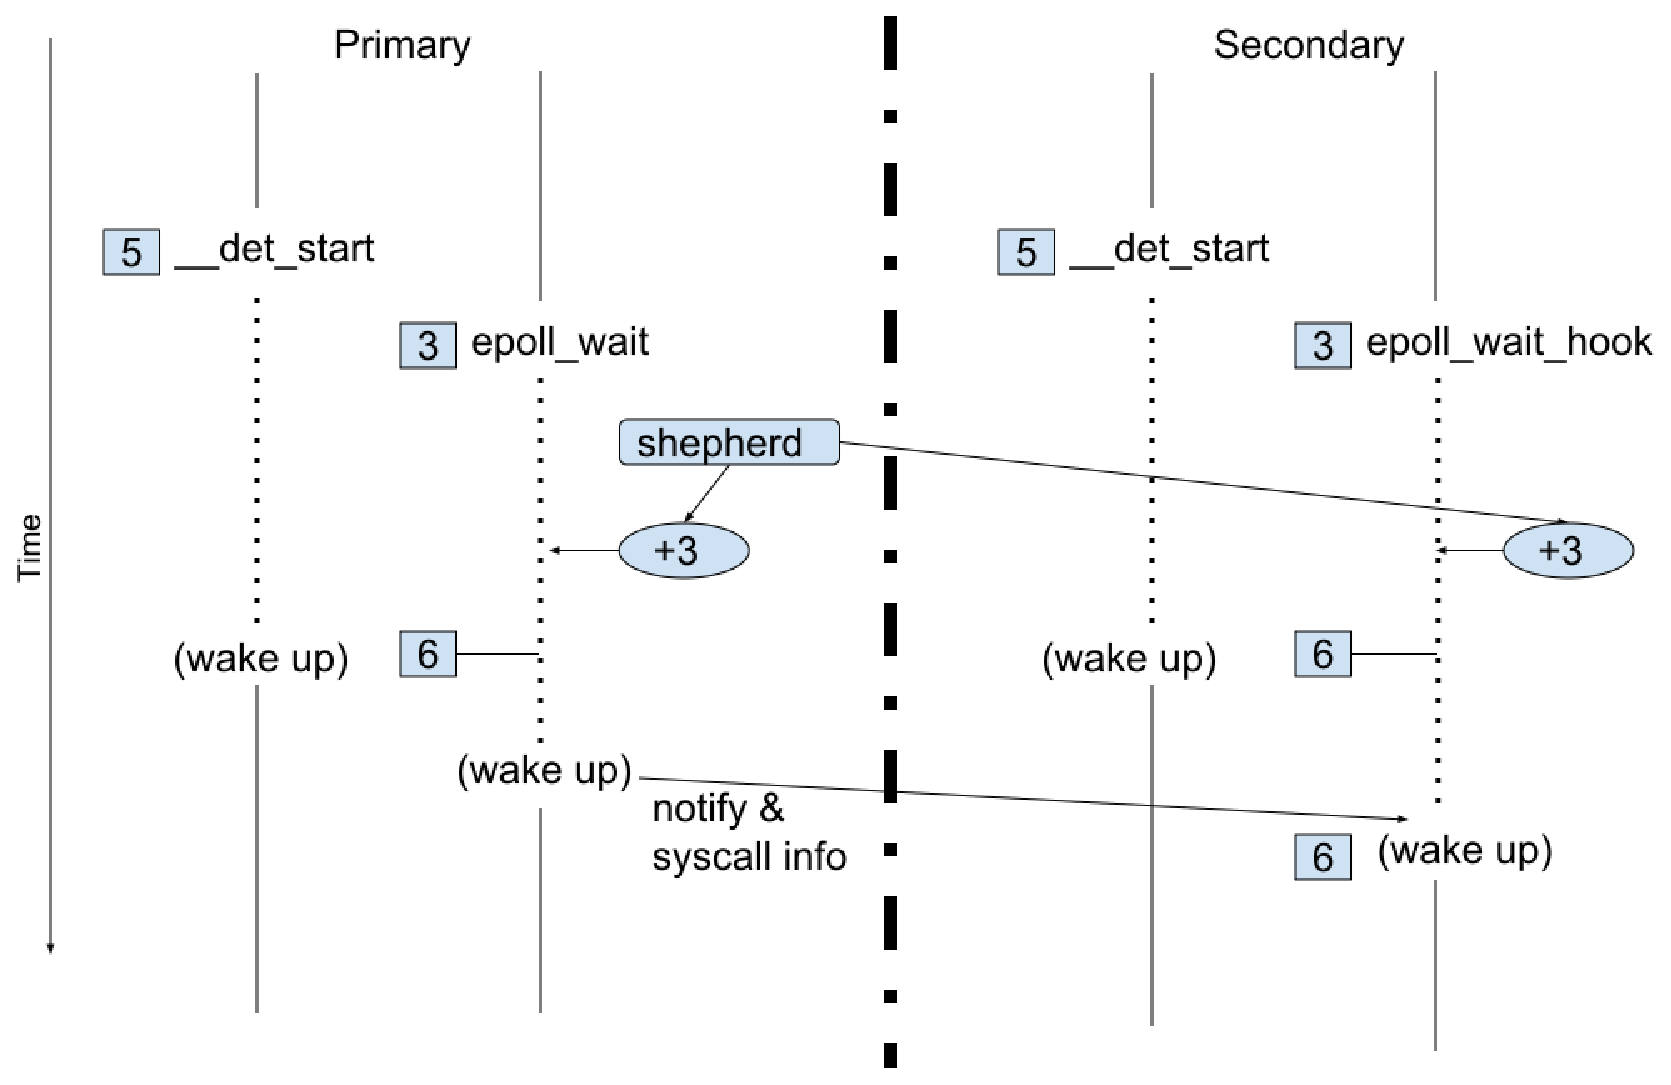
\includegraphics[width=0.8\columnwidth]{figures/tickbump}
\caption{An example of tick bumping}
\label{f:tick_bump}
\end{figure}

In order to let the token passing keep going with those blocking system calls, we need a way to keep bumping those thread's logical time while they are sleeping, a "Tick Shepherd" is implemented to dynamically bump the logical time of the threads that are sleeping in such system calls. The Tick Shepherd is a kernel thread which is mostly sleeping in the background, whenever the token is passed on to a thread that is sleeping on external events or a thread is going to sleep with the token, the shepherd will be woken up to increase the sleeping thread's logical time and send the increased value to the replica. In the meanwhile the corresponding system call on the replica will be blocked at the entry point, and bumps its logical time according to the information from the primary. The syscall on the secondary doesn't proceed until the primary returns from the syscall. In this way we can make sure that when both of the syscalls wake up from sleeping, all the replicas will end up with a consistent state, in terms of logical time. The Tick Shepherd will keep bumping sleeping tasks logical time until for a given period the state of all the tasks comes to a stable point, where nobody makes a single syscall. After that, it will go back to sleep again.


Figure~\ref{f:tick_bump} shows an example of how Tick Shepherd works in action. In this example, tick shepherd detects the token is on a thread sleeping in epoll\_wait, so it bumps its tick by 3 and sends this info to the secondary so that the token can leave this thread. And after the primary returns from epoll\_wait, it sends a message to the secondary, so that the corresponding thread can start to execute its epoll\_wait and uses the output from the primary as its own output.


We only let Tick Shepherd to bump the system calls that for sure will be called for deterministic times, the current implementation covers all the major I/O related system calls.

\section{Eliminate Deadlocks} \label{sec:edeadlock}
% cite futex and glic here
With wrapping all the pthread\_mutex\_lock with our deterministic system calls, there is a potential risk of having deadlocks. Serializing all the lock acquisitions with our implementation basically means putting a giant global mutex lock around every lock acquisition. As shown in Figure~\ref{fig:deadlock}, Thread 2 has a lower logical time and try to acquire the mutex(b), however mutex(b) is contended, as a result Thread 2 will call futex\_wait and put the thread into sleep until mutex(b) is released by someone else. At this point, Thread 2 will never increase its logical time until mutex(b) is released. So Thread 1 will never goes through the \_\_det\_start, and it will never unlock mutex(b), which means Thread 2 will never be woken up.

Since we already know that a contented mutex will call futex\_wait to wait for a unlock event, the solution to this deadlock problem is to temporary remove the thread in futex\_wait out of the deterministic schedule, and add it back when it returns from futex\_wait. In the example of Figure~\ref{fig:deadlock}, Thread 1 will be able to proceed its \_\_det\_start and keep executing. In order to not to break the determinism, we guarantee the following:
\begin{itemize}
\item We guarantee that the waiting queue in futex\_wait is strictly FIFO, which means the wakeup sequence will be the same as the sequence of getting into futex\_wait. Since the latter one is ensured by our \_\_det\_start, with this hack to futex, the wake up sequence from futex\_wait will be the same sequence determined by previous \_\_det\_start. This is implemented by fixing the priority of each futex object, so that the priority queue inside futex\_wait can behave like a FIFO queue.
\item We guarantee that when waking up from a futex\_wait, the thread always waits for the token before returning to the user space. With this implemented, the timing (in terms of logical time) of getting out of a contended pthread\_mutex\_lock will be deterministic. This is implemented by adding a \_\_det\_start after the wake up point of futex\_wait.
\end{itemize}

\begin{figure}
\centering
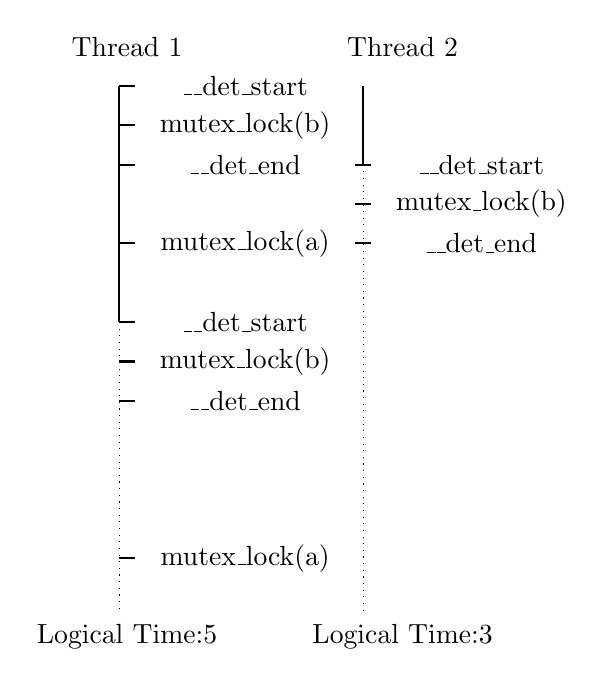
\begin{tikzpicture}
   \draw[thick] (-0.1,4) --  (-0.1,7); 
   \draw[dotted] (-0.1,4) --  (-0.1,0.3);
   
   \node[align=right] at (0,7.5) {Thread 1};
   
   \node[align=right] at (1.5,7) {\_\_det\_start};
   \draw[thick] (-0.1,7) -- (0.1,7);
   \node[align=right] at (1.5,6.5) {mutex\_lock(b)};
   \draw[thick] (-0.1,6.5) -- (0.1,6.5);
   \node[align=right] at (1.5,6) {\_\_det\_end};
   \draw[thick] (-0.1,6) -- (0.1,6);
   \node[align=right] at (1.5,5) {mutex\_lock(a)};
   \draw[thick] (-0.1,5) -- (0.1,5);      
   
   \node[align=right] at (1.5,4) {\_\_det\_start};
   \draw[thick] (-0.1,4) -- (0.1,4);
   \node[align=right] at (1.5,3.5) {mutex\_lock(b)};
   \draw[thick] (-0.1,3.5) -- (0.1,3.5);
   \node[align=right] at (1.5,3) {\_\_det\_end};
   \draw[thick] (-0.1,3) -- (0.1,3);
   \node[align=right] at (1.5,1) {mutex\_lock(a)};
   \draw[thick] (-0.1,1) -- (0.1,1);   
   \node[align=right] at (0,0) {Logical Time:5};
      %show thread 1 holds the lock previously

   \draw[thick] (3,6) --  (3,7); 
   \draw[dotted] (3,6) --  (3,0.3);
   
   \node[align=right] at (3.5,7.5) {Thread 2};
   \node[align=right] at (4.5,6) {\_\_det\_start};
   \draw[thick] (2.9,6) -- (3.1,6);
   \node[align=right] at (4.5,5.5) {mutex\_lock(b)};
   \draw[thick] (2.9,5.5) -- (3.1,5.5);
   \node[align=right] at (4.5,5) {\_\_det\_end}; 
   \draw[thick] (2.9,5) -- (3.1,5);   
   \node[align=right] at (3.5,0) {Logical Time:3};
\end{tikzpicture}
\caption{An example of deadlock}
\label{fig:deadlock}
\end{figure}

\section{Related Work}
Deterministic systems have been studied for a long time. From the implementation perspective view, they can be categorized into 4 different genres: language level, runtime level, OS level and architectural level.

% Use subsections to address each work
% To be fullfilled

Clik++~\cite{leiserson2010cilk++} is an parallel extension to C++ which makes creating parallel program easier. This extension provides a property that can indicate threads to be executed in a serial way, so that the determinism can be ensured. Grace \cite{berger2009grace} is also a C++ extension that adds a fork-join parallel schema to C++, it enforces the determinism of the execution with its underlying language runtime. Both of them are very limited to a specific parallel programming model, and existing applications need to be rewritten to achieve determinism.

Kendo\cite{olszewski2009kendo}, Parrot\cite{cui2013parrot} and Dthreads\cite{liu2011dthreads} provide runtime substitutions for pthread library. By making pthread synchronizations to be deterministic, any race-free pthread-based application can be executed in a deterministic way. They are easy to be applied onto existing applications. However they are limited to pthread only applications. Although Melchior can only make pthread to run deterministically in an automatically way, a developer is always free to use the runtime system calls to hand tune any type of parallel applications to make them deterministic. Among these three, Kendo uses the same deterministic scheduling policy as Melchior. However it relies on hardware counters to keep track of the program's progress in runtime, given the fact that hardware counters could be non-deterministic\cite{weaver2008can}, we doubt the determinism  of Kendo in some cases. DMP\cite{devietti2009dmp} provides an OS layer to make any program running on top of it deterministic, which is applicable for all kinds of parallel programming models. However DMP's overhead is too high due to massive trapping to shared memory accesses. We synchronization provided by the programming model, this could be unnecessary.

In \cite{segulja2012architectural}, an architectural solution is proposed. It's a hardware layer between the CPU core and memory hierarchy, the goal is to track all the memory access and does versioning on the memory operations. By doing deterministic submission to the memory hierarchy, it ensures the determinism of the parallel execution. Although it's a promising solution which is totally transparent to the upper layer, it's not usable out of box in recent years. 
\chapter{Nigoki: Schedule Replication} \label{chap:schedrep}
In chapter ~\ref{chap:detexec} we described using a deterministic system to ensure the applications on the primary and secondary replica can have the same thread interleaving. The major advantage of the deterministic system is that we can minimize the communication between the replicas. However the downside is that we need to precisely adjust the logical time to maintain decent parallelism for multithreaded applications. We showed various solutions to balance the logical time because we need to keep the execution to be fast and deterministic. If all the burdens come from being deterministic, can we break the determinism once for all but still keep the replicas to be synchronized? The answer is yes.

In this chapter we present Nigoki\footnote{Means Unit 2, in Japanese}: Schedule Replication. In this replication mode, we break the determinism entirely and use messages to synchronize every single synchronization primitives between the primary and replica.

For an application that has massive number of synchronization primitives, this approach might introduce overheads from the communication. Any latency in the the messaging will cause the secondary to fall behind the primary. Fortunately, our system is for inter-kernel replication, and Popcorn Linux provides a messaging layer with relatively low latency (basically memcpy from one kernel to another). As a result having massive massages between replicas won't put too much overhead to the replication.

% !!!!!!!!!put this into conclusion
% \begin{figure}
% \centering
% 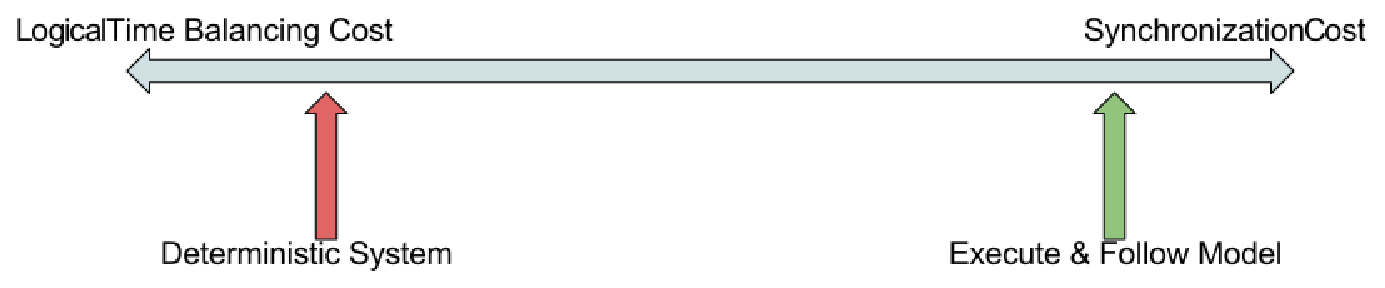
\includegraphics[width=0.8\columnwidth]{figures/tradeoff}
% \caption{Trade off between two algorithms}
% \label{f:tradeoff}
% \end{figure}

\section{Execute-Log-Replay}
Before we get into the detail of this algorithm, let us revisit some important properties that are provided by the deterministic system.

\begin{itemize}
\item Serialization of deterministic areas. (The code region between detstart and detend).
\item Same total order of getting into deterministic areas on primary and secondary.
\end{itemize}

The first property is guaranteed by the fact that the logical time will not change during the execution of a deterministic area, and the second property is guaranteed by increasing the logical time in a same way on both primary and replica. As long as these two properties are guaranteed, the thread interleaving on both primary and secondary are sure to be the same (also for tick bump). By following this paradigm, in our Schedule Replication mode, we guarantee these two properties with the following approaches:

\begin{itemize}
\item Serialize deterministic areas with a global mutex on both primary and secondary.
\item Log the sequence of getting into deterministic areas on the primary and replay it on the secondary.
\end{itemize}

\begin{figure}
\begin{lstlisting}[numbers=left, frame=single, basicstyle=\small, breaklines]{schedrep}
/*
 * Definitions:
 * ns: current popcorn namespace
 * ns->global_mutex: global_mutex in current namespace
 * ns->seq: global sequence number Seq_global
 * current->seq: task sequence number Seq_thread
 * current->ft_pid: replicated task unique identifier
 */
void __det_start()
{
    if (is_secondary(current))
        wait_for_sync(current->seq, 
            ns->seq, current->ft_pid);
    lock(ns->global_mutex);
    current->ft_det_state = FT_DET_ACTIVE;
}
void __det_end()
{
    if (is_primary(current))
        send_sync(current->seq, 
            ns->seq, current->ft_pid);
    current->seq++;
    ns->seq++;
    current->ft_det_state = FT_DET_INACTIVE;
    unlock(ns->global_mutex);
}
\end{lstlisting}
\caption{Simplified implementation of system calls for schedule replication}
\label{f:schedrep_c}
\end{figure}

% explain something for tha variables
% reference to ft_pid
% why I dont need to handle I/O

Here we still use \detstart\ and \detend\ to wrap around a code section that needs to be synchronized with the replica. Figure~\ref{f:schedrep_c} shows a simplified version of \detstart\ and \detend\ in Schedule Replication.  Every thread in the namespace maintains a sequence number $Seq_{thread}$ and the entire namespace maintains a sequence number $Seq_{global}$. On the primary, \detstart\ simply locks the global mutex, \detend\ unlocks the global mutex, sends a tuple of $< Seq_{thread}, Seq_{global}, ft\_pid >$ to the secondary and then increase the value of $Seq_{global}$ and $Seq_{thread}$. On the secondary, \detstart\ blocks until it receives a $< Seq_{thread}, Seq_{global}, ft\_pid >$ tuple corresponds to its caller thread, then holds the global mutex, and \detend\ increases $Seq_{global}$ and $Seq_{thread}$, then release the global mutex.

Figure~\ref{f:scherep} shows an example of how Schedule Replication works in action. In this example, T1 on the primary reached \detstart\ first and acquired the global mutex, which blocked T2 from getting into its \detstart\. After the primary reached \detend\, the global mutex is released and T2 was able to proceed. On the secondary, both T1' and T2' got blocked on \detstart\ at the beginning, no matter which one reached its \detstart\ first. T1' was able to proceed after T1 on the primary reached \detend\ and sent the notification to the secondary. T2' proceeded in the same way as T1' did. With this, the timing of calling mutex\_lock on the primary and secondary are synchronized on the primary and secondary.

For each namespace on the secondary, we have a queue for logging the incoming schedule replication message from the primary. The Popcorn message handler for schedule replication message simply appends the message into the queue tail and \detstart\ waits on the queue head to become the schedule sequence that it needs. A crucial prerequisite for this mechanism is that the message in the queue shall preserve strict FIFO sequence. Otherwise an out-of-order message in the queue tail will cause a deadlock in the system, because no \detstart\ will find the matching message in the queue tail. Our implementation guarantees the correct order of the messages, i.e, the messages are put in the queue in a monotonic sequence by their global sequence number $Seq_{global}$.

\begin{itemize}
  \item The synchronization message is sent with the global mutex on hold, this guarantees the monotonic sequence from the sender side.
  \item The messaging layer is strictly FIFO, which will not re-order the messages in its buffer, this guarantees the monotonic sequence from the receiver side.
\end{itemize}

\begin{figure}
\centering
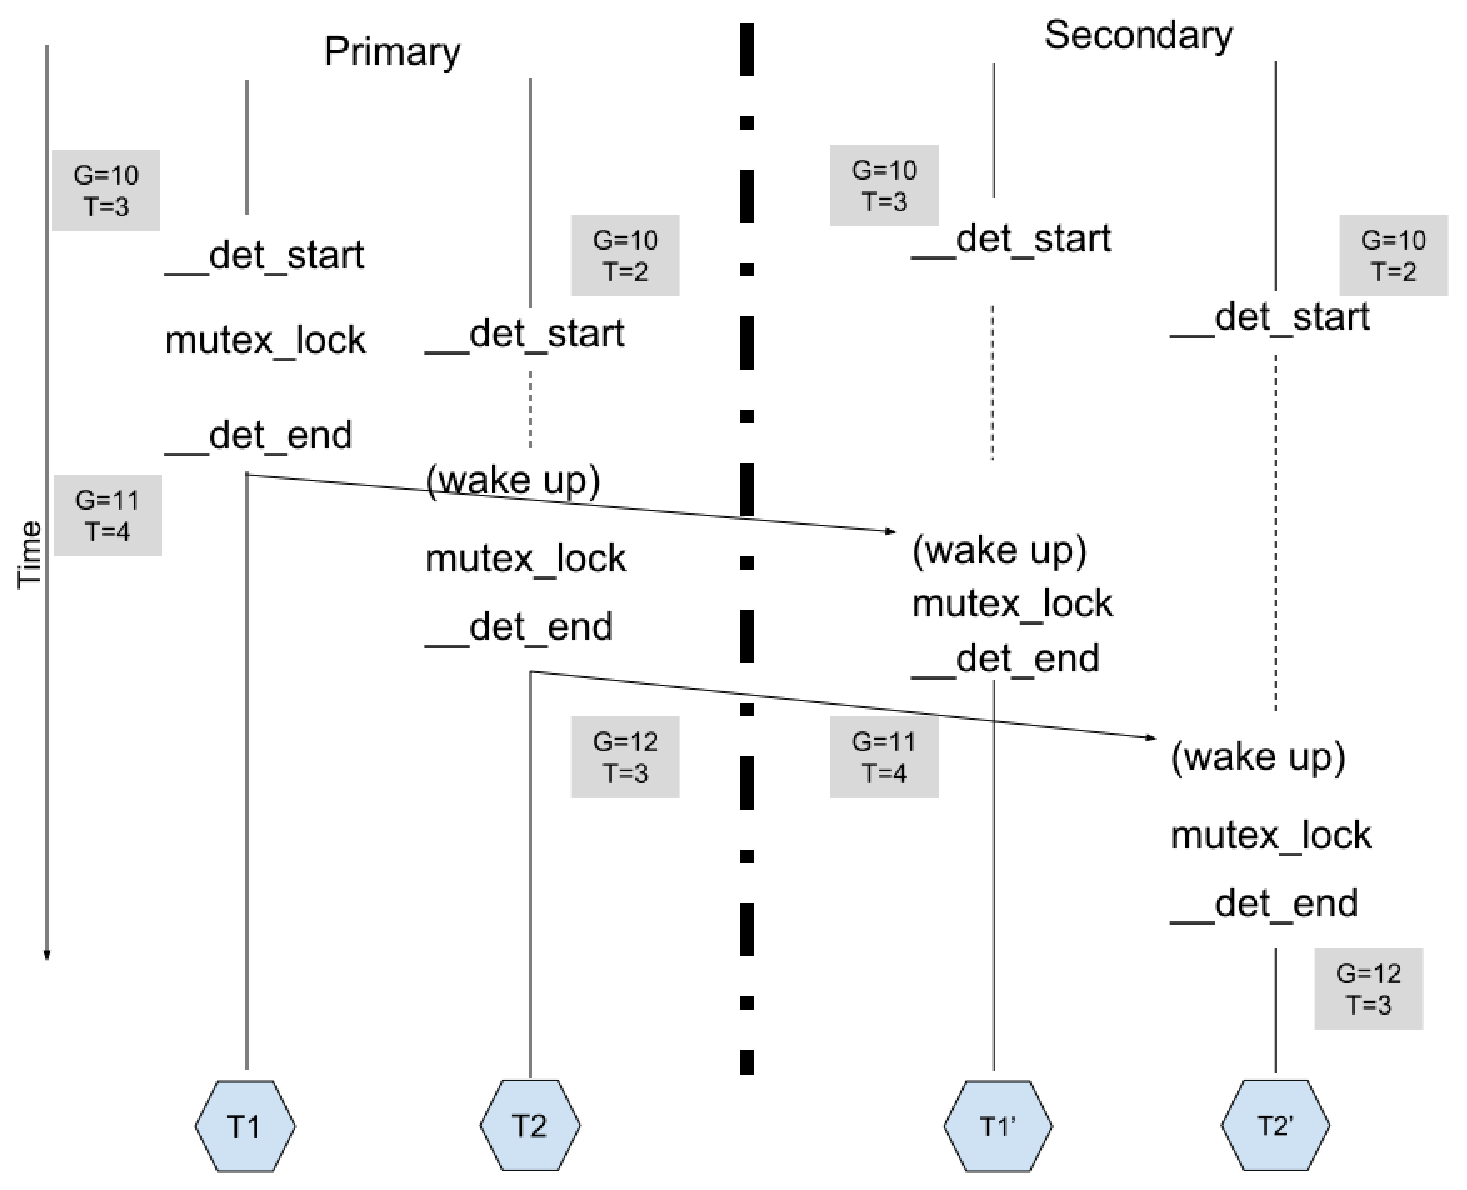
\includegraphics[width=0.9\columnwidth]{figures/sched_rep}
\caption{An example of Schedule Replication}
\label{f:scherep}
\end{figure}

\subsection{Eliminate Deadlocks} \label{sec:rdeadlock}
As we mentioned in Section~\ref{sec:edeadlock}, wrapping all the lock acquisitions with \detstart\ and \detend\ will occur the same deadlock issue, the reason is similar to the case in the Deterministic Execution because we don't release the lock acquisition order when the mutex is contended. The solution in Schedule Replication is similar to what we did in the Deterministic Execution, upon getting into sleep in futex, we release the global mutex and re-acquire it when it wakes up from futex. The futex modification mentioned in Section~\ref{sec:edeadlock} is also applied in this case to ensure the determinism of waking up from futex.

\section{Related Work}
Several previous works also presented the idea of not using a deterministic system for replication. Midas~\cite{slember2006static} points out the non-determinism from both the thread-interleaving and system call outputs, and utilizes a compiler framework to trap those non-deterministic points. The primary records the output of trapped points and replay them on the replica. Rex~\cite{guo2014rex} presents the same idea of logging the lock sequences on the primary and replay it on the replicas. It utilizes Paxos~\cite{lamport2001paxos} to provide a consistent sequence of requests and locks across all the replicas. Comparing to our solution, the advantage of Rex is that it is able to use partial order lock synchronization to provide decent parallelism for different lock acquisitions. But the downside is that both of the solutions are not transparent enough. In Rex, applications need to be manually modified to adopt Rex. (300-500 lines of changes for each application, according to the evaluation part of the paper.) Moreover, both solutions cannot deal with non-determinism comes from an external library.

A more aggressive idea is not synchronizing the execution sequence at all. EVE~\cite{kapritsos2012all}, Recspec~\cite{lee2010respec} and Zyzzyva~\cite{kotla2007zyzzyva} present the idea of running the replica speculatively without synchronizing the thread-interleaving. All of them assume for most of time the replicas are able to produces the consistent output, but whenever the replica diverges, the diverged one is forced to roll-back to a previous consistent state. Compare to our solution, EVE is implemented in JAVA and needs a good amount of manually annotation work to the applications, Zyzzyva seems to be highly customized and did not show evaluation for real world applications. For Recspec, it runs the application and the replicated one inside the same OS, which does not meet the requirement of our use case.
\chapter{Additional Runtime Support}
\section{Synchronization Exclusion}
\section{Syscall Synchronization}
\section{Modified Pthread Library}
\chapter{Evaluation}

In this chapter we will show some experiment results of our system. We will use various applications which will cover all the aspects of our implementation include thread interleaving synchronization, application instrumentation and system call synchronization. With all the evaluation, we will answer the following questions:

\begin{itemize}
  \item Correctness: Given the same input, can the primary and secondary consistently generate the same output?
  \item Performance: Compare to non-replicated execution, how much overhead is introduced by our system?
  \item Overhead: What do we need to pay for doing replication?
\end{itemize}
% Evaluation factors:
% 1. Lock count & pcnmsg count for schedule part
% 2. Breakdown
% 3. Absolute time

\paragraph{Evaluation Setup} All experiments were run on a server machine with 4 AMD Opteron 6376 Processors (16 cores each, 2.3Ghz), which is 64 cores in total. The total RAM is 128GB. Our Popcorn Linux kernel was installed on Ubuntu 12.04 LTS. We partitioned the hardware resources into half, one for the primary and one for the secondary. Each of them has the full control of their own 32 cores and 64GB RAM. The machine comes with a 1Gbps high speed connection. For benchmarking server applications, we used another server machine in the same rack, connected to the same switch, to act as the benchmark client.

\section{Racey}
We used a variant of racey~\cite{hillstress} to evaluate if our system can work correctly under various concurrent models, in other words, to evaluate the ability of maintaining the same thread-interleaving on all replicas. racey benchmark is a set of concurrent programs which read and write some shared data concurrently with various concurrent models. With a non-deterministic system, all the benchmark will create a different result during each different run. We use racey to validate if we can have the same thread interleaving on primary and secondary, which should lead the same output on both primary and secondary.

\paragraph{racey-guarded} racey-guarded has a global array, it uses pthread to create multiple threads and modify the global array concurrently. The access to the global array is protected by pthread\_mutex\_lock. We tested this one without any modification to the application. With both synchronization algorithms, we are able to create consistent results on the primary and secondary for over 100 consecutive runs.

\paragraph{racey-forkmmap} racey-forkmmap utilizes mmap to create a shared memory area, and uses fork to create multiple processes to read and modify the shared memory area. We 	added \_\_det\_start and \_\_det\_end around each access to the shared memory area. With both synchronization algorithms, we are able to create consistent results on the primary and secondary for over 100 consecutive runs.

\paragraph{racey-tcp} Based on the idea of racey, we developed racey-tcp to stress the determinism for network I/O related tasks. racey-tcp uses pthread to create multiple threads. One thread listens to the socket, whenever a new connection arrives, it puts the connection into a queue, other threads retrieve the connection from the queue, read the data on that connection and write the data into a file. For this benchmark, we wrapped the write system call for writing to the file with \_\_det\_start and \_\_det\_end. With both synchronization algorithms, we are able to create consistent output file on the primary and secondary for over 2000 requests.

\section{PBZip2}
% 1. threading model
% 2. A table of lock and cond var count
% 3. A table of instrumented dettick count
PBZip2~\cite{gilchristparallel} is the parallel version of bzip2. The concurrent model of this application is a typical producer-consumer model, as shown in Figure~\ref{f:pbzip_model}. The FileReader thread reads the content of the file, break the input data into data chunks and put all the chunks into a queue. Worker threads get the data chunks from the queue and do the compression/decompression, after all put the produced data to another queue. The FileWriter will keep getting products from the queue and write them to the final zip file. Multiple pthread\_mutex\_lock and pthread\_cond\_wait functions are applied to provide the mutual exclusion to the access of the queues.

\begin{figure}
\centering
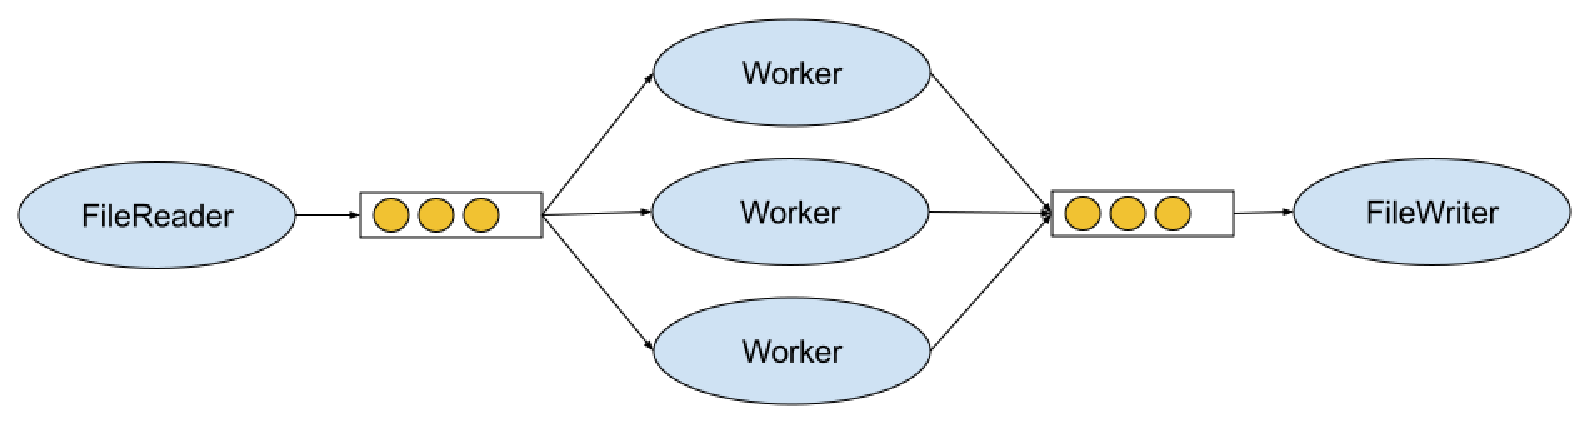
\includegraphics[width=0.8\columnwidth]{figures/pbzip2_model}
\caption{pbzip2 concurrent model}
\label{f:pbzip_model}
\end{figure}

For PBZip2, the time consuming part is the place where it calls the libz2 compression/decompression functions. In this benchmark, we utilized the execution time profiling instrumentation to balance the logical time for the deterministic execution, while for schedule replication nothing is modified. The benchmark is to compress a 177MB file with different thread counts, here we measure the performance with the total execution time reported by pbzip2. Other than that, no manually code modification was applied to the original source code.

Table~\ref{t:pbzip2_syscall} shows the system calls that are used by pbzip2, we only show the system calls that are tracked and synchronized by our system. In pbzip2,  gettimeofday is used for showing the time spent on the whole process, which it is not critical to the output of the application. However pthread\_cond\_timed\_wait also uses gettimeofday to calculate the timeout for the wait time, which is critical to the consistency of the execution.

\begin{table}
 \caption{Tracked system calls used by pbzip2}
\begin{center}
 \begin{tabular}{c | c}
 System Call & Use in the Application\\ \hline
 gettimeofday & Calculate execution time/pthread\_cond\_timed\_wait
 \end{tabular}
\end{center}
\label{t:pbzip2_syscall}
\end{table}

\paragraph{Correctness} For Deterministic Execution, any mismatch of the schedule will lead to different calling sequence of gettimeofday on the primary and secondary, which will result different reported execution time. For Schedule Replication, any mismatch of the schedule will lead the secondary waiting for a wrong schedule event forever. Neither of the case happened during the benchmark, the correctness of the replication thus proven.

\subsection{Results}

Figure~\ref{f:pbzip_b10_performance} shows the execution time of vanilla Linux, Deterministic Execution and Schedule Replication. Both replication modes achieved decent scalability. However, as we can see in Table~\ref{t:pbzip2_overall}, both algorithms' overhead increases with the thread count. One important overhead source for both replication modes comes from the serialization of all the synchronization primitives. With increasing thread count, the downside of breaking the parallelism of accessing those regions becomes more obvious.

For Deterministic Execution, another type of overhead comes from the logical time imbalance. As we mentioned before, the execution profiler takes the average execution time of basicblocks. However the execution time may vary during the actual run, especially for those basic blocks with file I/O, which has non-determinisitc execution time. Although the instrumented pbzip2 showed decent scalbility, the performance still could have been better if we could increase the logical time more precisely.

%different block sizes
\begin{figure}
\centering
\includegraphics[width=0.8\columnwidth]{figures/pbzip2_b10}
\caption{pbzip2 performance}
\label{f:pbzip_b10_performance}
\end{figure}

\begin{table}
\caption{pbzip2 Overall Overhead of Each Replication Mode}
\begin{center}
 \begin{tabular}{c | c | c}
Thread count & Deterministic Execution & Schedule Replication \\ \hline
 2 & 14.27\% & 0.89\% \\ \hline
 4 & 29.47\% & 4.08\% \\ \hline
 8 & 44.77\% & 6.72\% \\ \hline
 16 & 54.44\% & 24.7\% \\ \hline
 24 & 63.39\% & 36.3\% \\ \hline 
 \end{tabular}
\end{center}
\label{t:pbzip2_overall}
\end{table}

\subsection{Message Breakdown}
Figure~\ref{f:pbzip2_msg} shows the number of messages that were used during the benchmark. In all the figures, "Syscall Messages" is the message count for synchronizing system calls, "Network Messages" mean the message count for replicating the network stack, and "Schedule Messages" means the messages for Tick Shepherd in Deterministic Execution, while in Schedule Replication this stands for the messages for logging the execution sequence. This result is expected as we assume that Deterministic Execution doesn't require too much communication between the replicas. Here all the system call messages are for gettimeofday, and most of them are from pthread\_cond\_timed\_wait. In pbzip2, pthread\_cond\_timed\_wait is used by Worker threads to wait for available data chunks. An interesting finding is that for the same benchmark Deterministic Execution invoked less system calls than Schedule Replication. This is because for Deterministic Execution there is a minor logical time imbalance issue, where the FileReader and FilerWriter had more chance to run compare to Worker threads. In this situation, whenever a Worker thread has chance to run, it is very likely to find an available data chunk in the queue, thus no need to call pthread\_cond\_timed\_wait. However for Schedule Replication, the arbitrary thread interleaving causes the Worker threads having more chance waiting on an empty queue, which leads to more invocation to pthread\_cond\_timed\_wait.
\begin{figure}
\centering
\includegraphics[width=1\columnwidth]{figures/pbzip2_msg}
\caption{pbzip2 messages}
\label{f:pbzip2_msg}
\end{figure}

\section{Mongoose Webserver}
% 1. threading model
% 2. A table of lock and cond var count

Mongoose~\cite{mongoose} is a compact multithreaded webserver. The concurrent model is shown in Figure~\ref{f:mongoose_model}. The MasterThread opens a listening socket, uses poll to wait for the incoming connections on the listening socket. Whenever a connection comes, the MasterThread accepts it and put the file descriptor to a queue. WorkerThreads get the connections from the queue and make the response to the clients. Table~\ref{t:mongoose_syscall} shows the system calls that are used by mongoose. The non-deterministic points in mongoose comes from both the thread-interleaving and system call output: diverged thread-interleaving leads to WorkerThreads handling incorrect sockets; diverged system call output leads to incorrect socket state and output value.

We used ApacheBench to stress test mongoose with different file sizes and different mongoose thread counts. For each benchmark set, we used 100 concurrent connections to make 20000 requests in total. For our benchmark on Deterministic Execution, since the file I/O is set to be blocking in mongoose and we do not track file I/O with Tick Shepherd, we manaully added a \dettick\ right before the file I/O system call with an optimal value (only 1 line). Other than that, nothing was changed for mongoose.

\begin{figure}
\centering
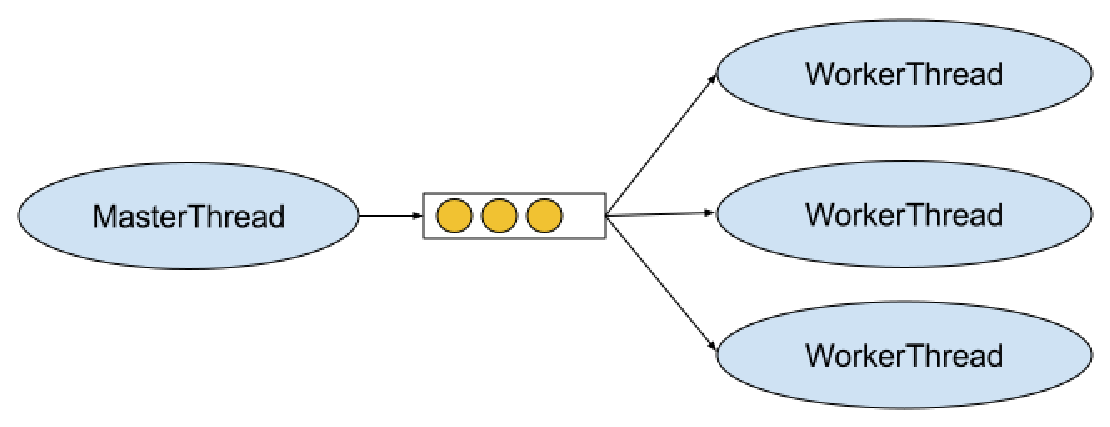
\includegraphics[width=0.6\columnwidth]{figures/mongoose_model}
\caption{mongoose concurrent model}
\label{f:mongoose_model}
\end{figure}

%Given mongoose's concurrent model, we can see that different file size will affect the frequency of acquiring locks. In this way we can figure out how will two algorithm perform under different lock acquisition load. Also, different thread counts can reflect the scalability of our system.
%cite ab

\begin{table}
\caption{Tracked system calls used by mongoose}
\begin{center}
 \begin{tabular}{c | c}
System Call & Use in the Application\\ \hline
 time & Generate HTTP header  \\ \hline
 poll & Wait for accept, read and write
 \end{tabular}
\end{center}
\label{t:mongoose_syscall}
\end{table}

\paragraph{Correctness} For both replication mode, any mismatch will lead to either different thread handling different socket, or divergence in the HTTP responses. Neither of the case happened during the benchmark, the correctness of the replication thus proven.

\subsection{Results}
\begin{figure}
\centering
\includegraphics[width=0.7\columnwidth]{figures/mg_throughput_50k}
\caption{mongoose performance for 50KB file requests}
\label{f:mg_50k}
\end{figure}
\begin{figure}
\centering
\includegraphics[width=0.7\columnwidth]{figures/mg_throughput_100k}
\caption{mongoose performance for 100KB file requests}
\label{f:mg_100k}
\end{figure}
\begin{figure}
\centering
\includegraphics[width=0.7\columnwidth]{figures/mg_throughput_200k}
\caption{mongoose performance for 200KB file requests}
\label{f:mg_200k}
\end{figure}

\begin{table}
\caption{Mongoose Overall Overhead of Each Replication Mode}
\begin{center}
 \begin{tabular}{c | c | c}
Thread Count & Deterministic Execution & Schedule Replication \\ \hline
 4 & 25.22\% & 1.35\% \\ \hline
 8 & 15.72\% & 0.27\% \\ \hline
 16 & 9.82\% & 0.23\% \\ \hline
 \end{tabular}
\end{center}
\label{t:mongoose_overall}
\end{table}

Figure ~\ref{f:mg_50k}, ~\ref{f:mg_100k} and ~\ref{f:mg_200k} show the performance under different workload, and Table ~\ref{t:mongoose_overall} shows the overall overhead of each replication mode. Deterministic Execution's overhead becomes lower as the thread count goes up, but still higher than Schedule Replication. This is due to blocking socket write and file I/O  operations. Because the time spent inside those blocking I/O varies all the time, our manually inserted \dettick\ couldn't precisely increase the logical time for every call, as a result we had to suffer the performance loss from logical time imbalance. In the meanwhile, Schedule Replication showed near zero overhead compare to the baseline.

Unlike pbzip where the overhead becomes higher when the thread count increases, mongoose's overhead decreases with more number of threads. This is because monoogse only has two condition variables and one mutex lock, the side effect of serializating pthread primitives is minimal and the performance thus can scale.

\subsection{Message Breakdown}
Figure~\ref{f:mg_msg_50k}, Figure~\ref{f:mg_msg_100k} and Figure~\ref{f:mg_msg_200k} show the breakdown of overall messages for each benchmark set. The notation is the same as the previous section. Where "Schedule Messages" means the messages for Tick Shepherd in Deterministic Execution, a in Schedule Replication this stands for the messages for logging the execution sequence.

Actually, we need much more messages for deterministic execution, which contradicts the assumption we made for Deterministic Execution. In mongoose, socket write and file I/O are blocking operations, and bigger network payload leads to more socket calls, thus we need more messages for the Tick Shepherd to synchronize the tick bumps. However for Schedule Replication, since the messages for scheduling only depends on the number of synchronization primitives, which totally depends on the number of requests (not the size), as a result, across all the benchmarks, the number of schedule messages for Schedule Replication show a near constant value across all the benchmarks.

\begin{figure}
\centering
\includegraphics[width=0.7\columnwidth]{figures/mg_msg_50k}
\caption{mongoose messages for 50KB file requests}
\label{f:mg_msg_50k}
\end{figure}
\begin{figure}
\centering
\includegraphics[width=0.7\columnwidth]{figures/mg_msg_100KB}
\caption{mongoose messages for 100KB file requests}
\label{f:mg_msg_100k}
\end{figure}
\begin{figure}
\centering
\includegraphics[width=0.7\columnwidth]{figures/mg_msg_200KB}
\caption{mongoose messages for 200KB file requests}
\label{f:mg_msg_200k}
\end{figure}
\section{Nginx Webserver}

Nginx~\cite{reese2008nginx} is a sophisticated webserver with multiple threading modes. In this benchmark we used the threadpool setup~\cite{nginxthreadpool} for our benchmark. As shown in Figure~\ref{f:nginx_model}, in this threading mode, the additional threads are only for doing file I/O operations. The MasterThread waits on the listening socket, whenever a file request is coming, it hands over the request into a queue. WorkerThreads get notified whenever a new request is coming and try to retrieve one task from the queue. Whenever the content of the requested file is loaded into memory by a WorkerThread, a handle will be put into another queue and the MasterThread will get notified. In the end, the MasterThread will retrieve the handle and send the content of the file back to the client. 

Table ~\ref{t:nginx_syscall} shows all the tracked system calls used by Nginx. All of the I/O operations are asynchronous and heavily relies on epoll mechanism. 

\begin{figure}
\centering
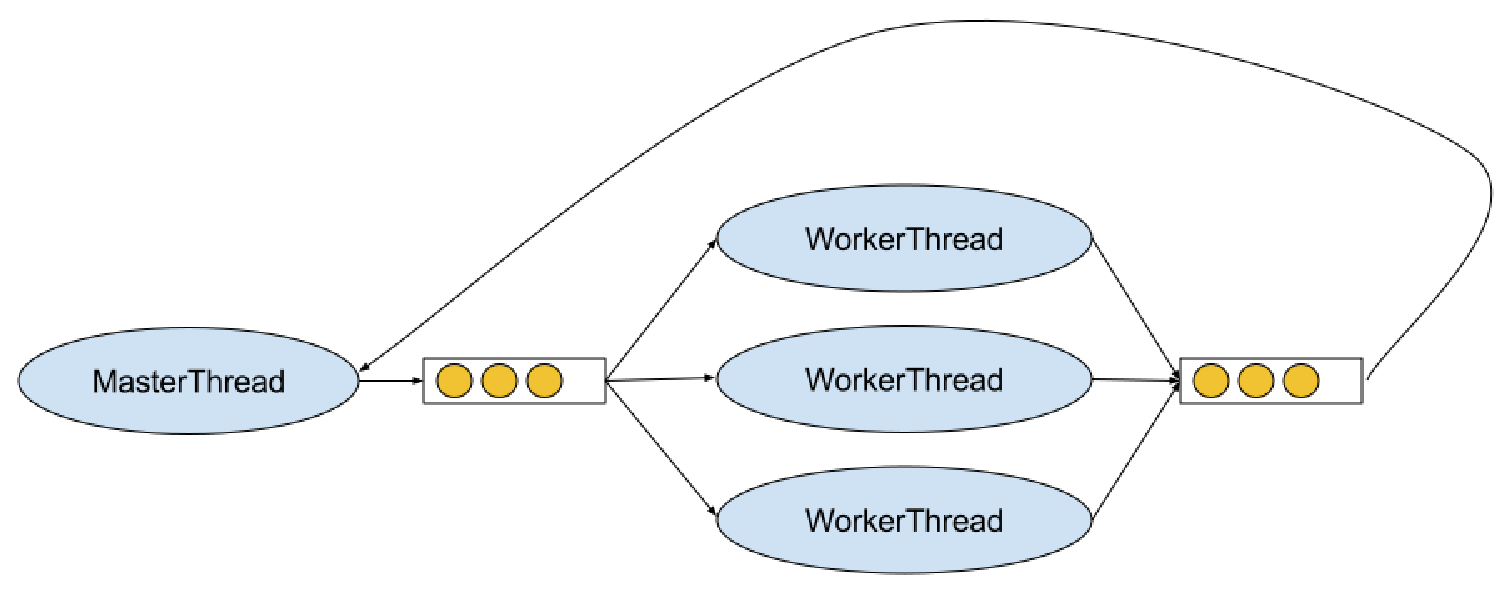
\includegraphics[width=0.8\columnwidth]{figures/nginx_model}
\caption{Nginx thread pool model}
\label{f:nginx_model}
\end{figure}

The same as mongoose, we used ApacheBench to stress test the server with different file sizes and different mongoose thread counts. For each benchmark set, we used 100 concurrent connections to make 20000 requests in total.

Nginx has multiple explicit atomic operations that might lead to non-deterministic results, here we applied \detstart\ and \detend\ around those operations to maintain the total order of those operations. Another non-deterministic part in Nginx is that it uses eventfd to communicate among threads. As we mentioned before, all inter-thread communication need to be deterministic on all the replicas, as a result, we applied \detstart\ and \detend\ around the read and write operations of eventfd to synchronize the total order of those operations. Other than that, no further modification were applied. In total, we added around 60 LOC to the original code.
%cite event fd here

\begin{table}
\caption{Tracked system calls used by nginx}
\begin{center}
 \begin{tabular}{c | c }
System Call & Use in the Application\\ \hline
 gettimeofday & Generate HTTP header\\ \hline
 epoll\_wait & Wait for accept, read and write
 \end{tabular}
\end{center}
\label{t:nginx_syscall}
\end{table}

\paragraph{Correctness} Similar to mongoose, any mismatch will lead to either different thread handling different socket, or divergence in the HTTP responses. Neither of the case happened during the benchmark, the correctness of the replication thus proven.

\subsection{Results}
\begin{figure}
\centering
\includegraphics[width=0.8\columnwidth]{figures/ng_throughput_50k}
\caption{nginx performance for 50KB file requests}
\label{f:ng_50k}
\end{figure}
\begin{figure}
\centering
\includegraphics[width=0.8\columnwidth]{figures/ng_throughput_100k}
\caption{nginx performance for 100KB file requests}
\label{f:ng_100k}
\end{figure}
\begin{figure}
\centering
\includegraphics[width=0.8\columnwidth]{figures/ng_throughput_200k}
\caption{nginx performance for 200KB file requests}
\label{f:ng_200k}
\end{figure}

\begin{table}
\caption{Nginx Overall Overhead of Each Replication Mode}
\begin{center}
 \begin{tabular}{c | c | c}
Thread Count & Deterministic Execution & Schedule Replication \\ \hline
 4 & 3\% & 1.07\% \\ \hline
 8 & 1.62\% & 1.96\% \\ \hline
 16 & 1.6\% & 1.31\% \\ \hline
 \end{tabular}
\end{center}
\label{t:nginx_overall}
\end{table}

The reason we see the result is not scaling (even for Linux) is because this threading mode for Nginx is only for concurrent file I/O. During our benchmark, we've already achieved the best of our filesystem even with lower thread counts, although all the threads were loaded, putting more threads won't increase the performance too much. However, the purpose of the benchmark is to show that how will different thread counts affecting our system's overhead (comparing to baseline), a non-scaling result still makes sense here.

Unlike mongoose, the result of Nginx showed both replication modes can achieve very small overhead. When we take a step back to deterministic execution, the major performance hurdle is the logical time imbalance, which happens when there are some time consuming code sections. However, since nginx fully utilizes asynchronous file and network I/O, everything is super fast. In the context of deterministic execution, we can say in Nginx there is no significant time consuming part that will cause logical time imbalance. Therefore Deterministic Execution can perform its best.

%On the other hand, the massive amount of messages used by Schedule Replication has put a more obvious overhead to the execution. That is why we are able to see Deterministic Execution can perform better.

\subsection{Message Breakdown}
\begin{figure}
\centering
\includegraphics[width=0.8\columnwidth]{figures/ng_msg_50KB}
\caption{nginx messages for 50KB file requests}
\label{f:ng_msg_50k}
\end{figure}
\begin{figure}
\centering
\includegraphics[width=0.8\columnwidth]{figures/ng_msg_100KB}
\caption{nginx messages for 100KB file requests}
\label{f:ng_msg_100k}
\end{figure}
\begin{figure}
\centering
\includegraphics[width=0.8\columnwidth]{figures/ng_msg_200KB}
\caption{nginx messages for 200KB file requests}
\label{f:ng_msg_200k}
\end{figure}
%The message breakdown has proved the analysis we made. Without any logical time imbalance, messaging and serilization are the only overhead sources for the system for Deterministic Execution.
Figure ~\ref{f:ng_50k}, figure ~\ref{f:ng_100k} and figure ~\ref{f:ng_100k} show the message break for our benchmark. As mention in the beginning of this section, Nginx needs more \detstart\ and \detend\ other than pthread primitives, so Schedule Replication uses way more messages than Deterministic Execution. Another interesting fact is that since asynchronous I/O operations are really fast in Nginx, in Deterministic Execution, the Tick Shepherd barely made a tick bump, which is also a reason that Deterministic Execution could perform much better than it was in mongoose. While in mongoose, almost every blocking I/O had at least one tick bump.

%\section{Redis Database Server}
%Redis is an in-memory database server. It uses a single thread to process requests, but it dynamically creates new threads to write the in-memory data to the disk. This benchmark is perfect for stressing the flexibility of dealing with dynamically spawned threads.

%For the performance test we used the redis-benchmark tool, we used the default benchmark parameter which will test all the operations. Each operation is tested for 10000 requests. We also have different number of concurrent clients to stress the server with different frequency of requests. We ran each setup for 5 times and took the average of the numbers.

%Redis uses an alternative memory allocator jemalloc, which contains some internal locks to ensure mutual exclusion for concurrent memory allocation. As mentioned in Section~\ref{sec:elision}, those lock acquisitions doesn't affect the output at all, so we modified the jemalloc's source code, to skip the synchronizations for those locks. Other than that, no further modification was made to the application.

%\subsection{Results}
%Figure~\ref{f:redis_2}, figure~\ref{f:redis_16} and figure~\ref{f:redis_64} show the  performance of redis with 2, 16 and 64 concurrent clients. Table~\ref{t:redis_overall} shows the overall overhead of each replication mode.

%The configuration was set to save the data every 10000 requests, which means for each benchmark of each operation, we will have one write back to the disk.

%\begin{figure}
%\centering
%\includegraphics[width=0.8\columnwidth]{figures/redis_2}
%\caption{redis benchmark with 10000 requests and 2 clients}
%\label{f:redis_2}
%\end{figure}

%\begin{figure}
%\centering
%\includegraphics[width=0.8\columnwidth]{figures/redis_16}
%\caption{redis benchmark with 10000 requests and 16 clients}
%\label{f:redis_16}
%\end{figure}

%\begin{figure}
%\centering
%\includegraphics[width=0.8\columnwidth]{figures/redis_64}
%\caption{redis benchmark with 10000 requests and 64 clients}
%\label{f:redis_64}
%\end{figure}

%\begin{table}
%\caption{Redis Overall Overhead of Each Replication Mode}
%\begin{center}
% \begin{tabular}{c | c | c}
%Client count & Deterministic Execution & Schedule Replication \\ \hline
% 2 & 30.38\% & 11.93\% \\ \hline
% 16 & 41.05\% & 26.94\% \\ \hline
% 64 & 39.66\% & 26.48\% \\ \hline
% \end{tabular}
%\end{center}
%\label{t:redis_overall}
%\end{table}

%\subsection{Message Breakdown}

\section{Discussion}
The selected benchmarks were used to stress different aspects of this project. Although there are still some optimizations to go, we still achieved decent overhead for different types of concurrent models and different application types. Here we will discuss some interesting issues during the benchmark and some findings from the results.

\subsection{Benchmark for Nginx's Multi-process Mode}
So far for all the marco benchmarks, we only showed benchmarks for multi-threaded applications. However our system also supports replication for multi-process applications (as we showed for racey microbenchmark). Nginx supports multi-worker mode, which spawns multiple worker processes, all of the worker processes wait on the listening socket together. Nginx implements the accept\_mutex ~\cite{nginxscalability}, which is lock across processes, to ensure an incoming request only wakes up one waiting worker. In order to figure out whether our replication works for this concurrent model or not, we manually instrumented the accept\_mutex acquisition with \detstart\ and \detend\ . During the benchmark, both primary and secondary were able to end up with the same state all the time. However no matter how many workers we put, it was always only one worker handling all the request. This is due to a relatively low workload we used in our benchmark. However, because of the limitation of our network card (1Gbps), we couldn't apply heavier workload to saturate the worker. With Nginx's design, the accept\_mutex mechanism will not pass the request to another worker if the current worker is not saturated. Which is the reason we only saw one worker handling all the requests.

Unlike the non-scaling result with the threadpool mode, where all the threads were fully loaded, the unbalanced workload in multi-worker mode seems not making any sense. As a result we didn't include the result in this chapter.

\subsection{Deterministic Execution's Dilemma}
For deterministic execution, a type of overhead comes from the calculation of the token (finding the task with minimal logical time). Current implementation requires O(N) time to decide which task should execute on next \detstart\ , where N is the number of threads. Every logical time update comes with such a computation process, more threads lead to more computation time.  As we can see from all the benchmarks, deterministic system always leads to a higher overhead when thread count increases. In a previous discussion ~\cite{bergan2011deterministic}, it is pointed out that all the existing deterministic systems, regardless of what type of deterministic algorithm (lockstep or wait for turn), this kind of global communication is inevitable. This also implies that deterministic might not be practical for highly concurrent application with highly intensive inter-thread communications (synchronization primitives). Webservers like mongoose and nginx have very simple inter-thread communication , so that we achieved decent overhead during the benchmark. But for more complicated applications with more different types of locks, we might face severe performance overhead.

\subsection{Which Replication Mode Should I Use?}
From all the benchmarks, we saw that some are better for Deterministic Execution and some are better for Schedule Replication. Figure~\ref{f:trade_off} shows the basic idea of what kind of price we are paying for different replication modes. For Deterministic Execution, if we are able to precisely balance the logical time, or there is no logical time imbalance problem (like Nginx), it is the choice. For Schedule Replication, since on Popcorn Linux, the cost of sending a message is under 2 microseconds, despite the huge amount of messages that Schedule Replication needs, the overall overhead from messaging can nearly be ignored. As long as the cost of sending messages keeps low, Schedule Replication is always the better choice.

\begin{figure}
\centering
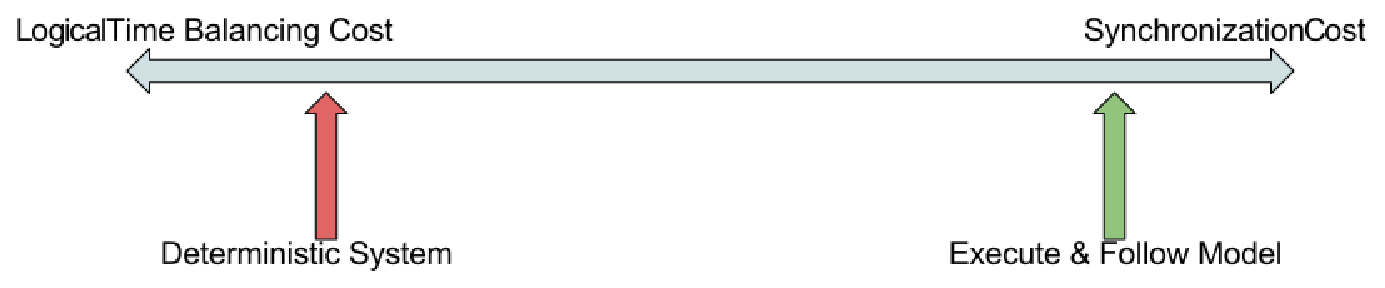
\includegraphics[width=1\columnwidth]{figures/tradeoff}
\caption{The tradeoff of two replication modes}
\label{f:trade_off}
\end{figure}
\chapter{Conclusion}
\section{Contributions}
\section{Future Work}
\subsection{Precise Tick Bump for Deterministic Execution}
The major overhead for Deterministic Execution is the imbalanced logical time, the more precise the logical time incremental is the less waiting time a task will need for waiting the token. In chapter ~\ref{chap:detexec} we described our solution with a profiling approach, but from the evaluation we see this is still not precise enough to have the best performance. While performance counters are not deterministic enough to do the job, Intel PT~\cite{intelpt} seems to be a promising approach to track the progress of the execution. 
\subsection{Pre-Lock Synchronization}
\subsection{Arbitrary Number Replicas}
%cite consensus here, mention paxos made transparent, rex
\subsection{Hybrid Replication}
%same, cite consensus here, mention paxos made transparent, rex
\section{Further Evaluation}

\input{bibliography}

\end{document}

